\documentclass[aspectratio=169,11pt]{beamer}

\usetheme{metropolis}

\usepackage{booktabs}
\usepackage{graphicx}
\usepackage{tikz}
\usepackage{appendixnumberbeamer}

% ── Colour palette ──────────────────────────
\definecolor{bg}{HTML}{33271E}
\definecolor{muted}{HTML}{8A7B94}
\definecolor{sage}{HTML}{8FBCB3}
\definecolor{lime}{HTML}{C8E88F}
\definecolor{cream}{HTML}{F6F4E8}
\definecolor{sand}{HTML}{C4956A}  % tantalum, matches the figures

% ── Apply palette to beamer elements ────────
\setbeamercolor{normal text}{fg=cream, bg=bg}
\setbeamercolor{alerted text}{fg=lime}
\setbeamercolor{example text}{fg=sage}

\setbeamercolor{frametitle}{fg=cream, bg=bg}
\setbeamercolor{title}{fg=cream, bg=bg}
\setbeamercolor{subtitle}{fg=sage}
\setbeamercolor{author}{fg=cream}
\setbeamercolor{institute}{fg=muted}
\setbeamercolor{date}{fg=muted}

\setbeamercolor{progress bar}{fg=sage, bg=bg!80!black}
\setbeamercolor{title separator}{fg=sage}

\setbeamercolor{block title}{fg=bg, bg=sage}
\setbeamercolor{block body}{fg=cream, bg=bg!85!black}

\setbeamercolor{block title alerted}{fg=bg, bg=lime}
\setbeamercolor{block body alerted}{fg=cream, bg=bg!85!black}

\setbeamercolor{item}{fg=sage}
\setbeamercolor{subitem}{fg=muted}

\setbeamercolor{footnote}{fg=muted}
\setbeamercolor{footnote mark}{fg=muted}

\setbeamercolor{standout}{fg=bg, bg=sage}

% ── Fonts ───────────────────────────────────
\setbeamerfont{frametitle}{series=\bfseries}

% ── Custom command for question emphasis ────
\newcommand{\audience}[1]{%
  \vspace{0.5em}%
  {\color{lime}\textbf{Question:}} {\color{cream}#1}%
}


\title{Critical Minerals, Governance and Armed Conflict}
\subtitle{Evidence from Africa}
\author{Elisa D'Amico \and P\"aivi Lujala}
\institute{University College Dublin \and University of Oulu}
\date{APSA Annual Meeting, 2026}

\begin{document}

\maketitle

% ═══════════════════════════════ QUESTION ═══════════════════════════════
\begin{frame}{The Question}
  \begin{columns}[c]
    \begin{column}{0.45\textwidth}
      {\Large\color{cream}
        When a critical mineral is found,\\[0.35em]
        does the violence around it depend on\\[0.35em]
        \textcolor{lime}{how that mineral is governed}?}
      \vspace{1.2em}

      {\color{muted}What varies is the \textbf{institutional regime}
      attached to the mineral.}
    \end{column}
    \begin{column}{0.55\textwidth}
      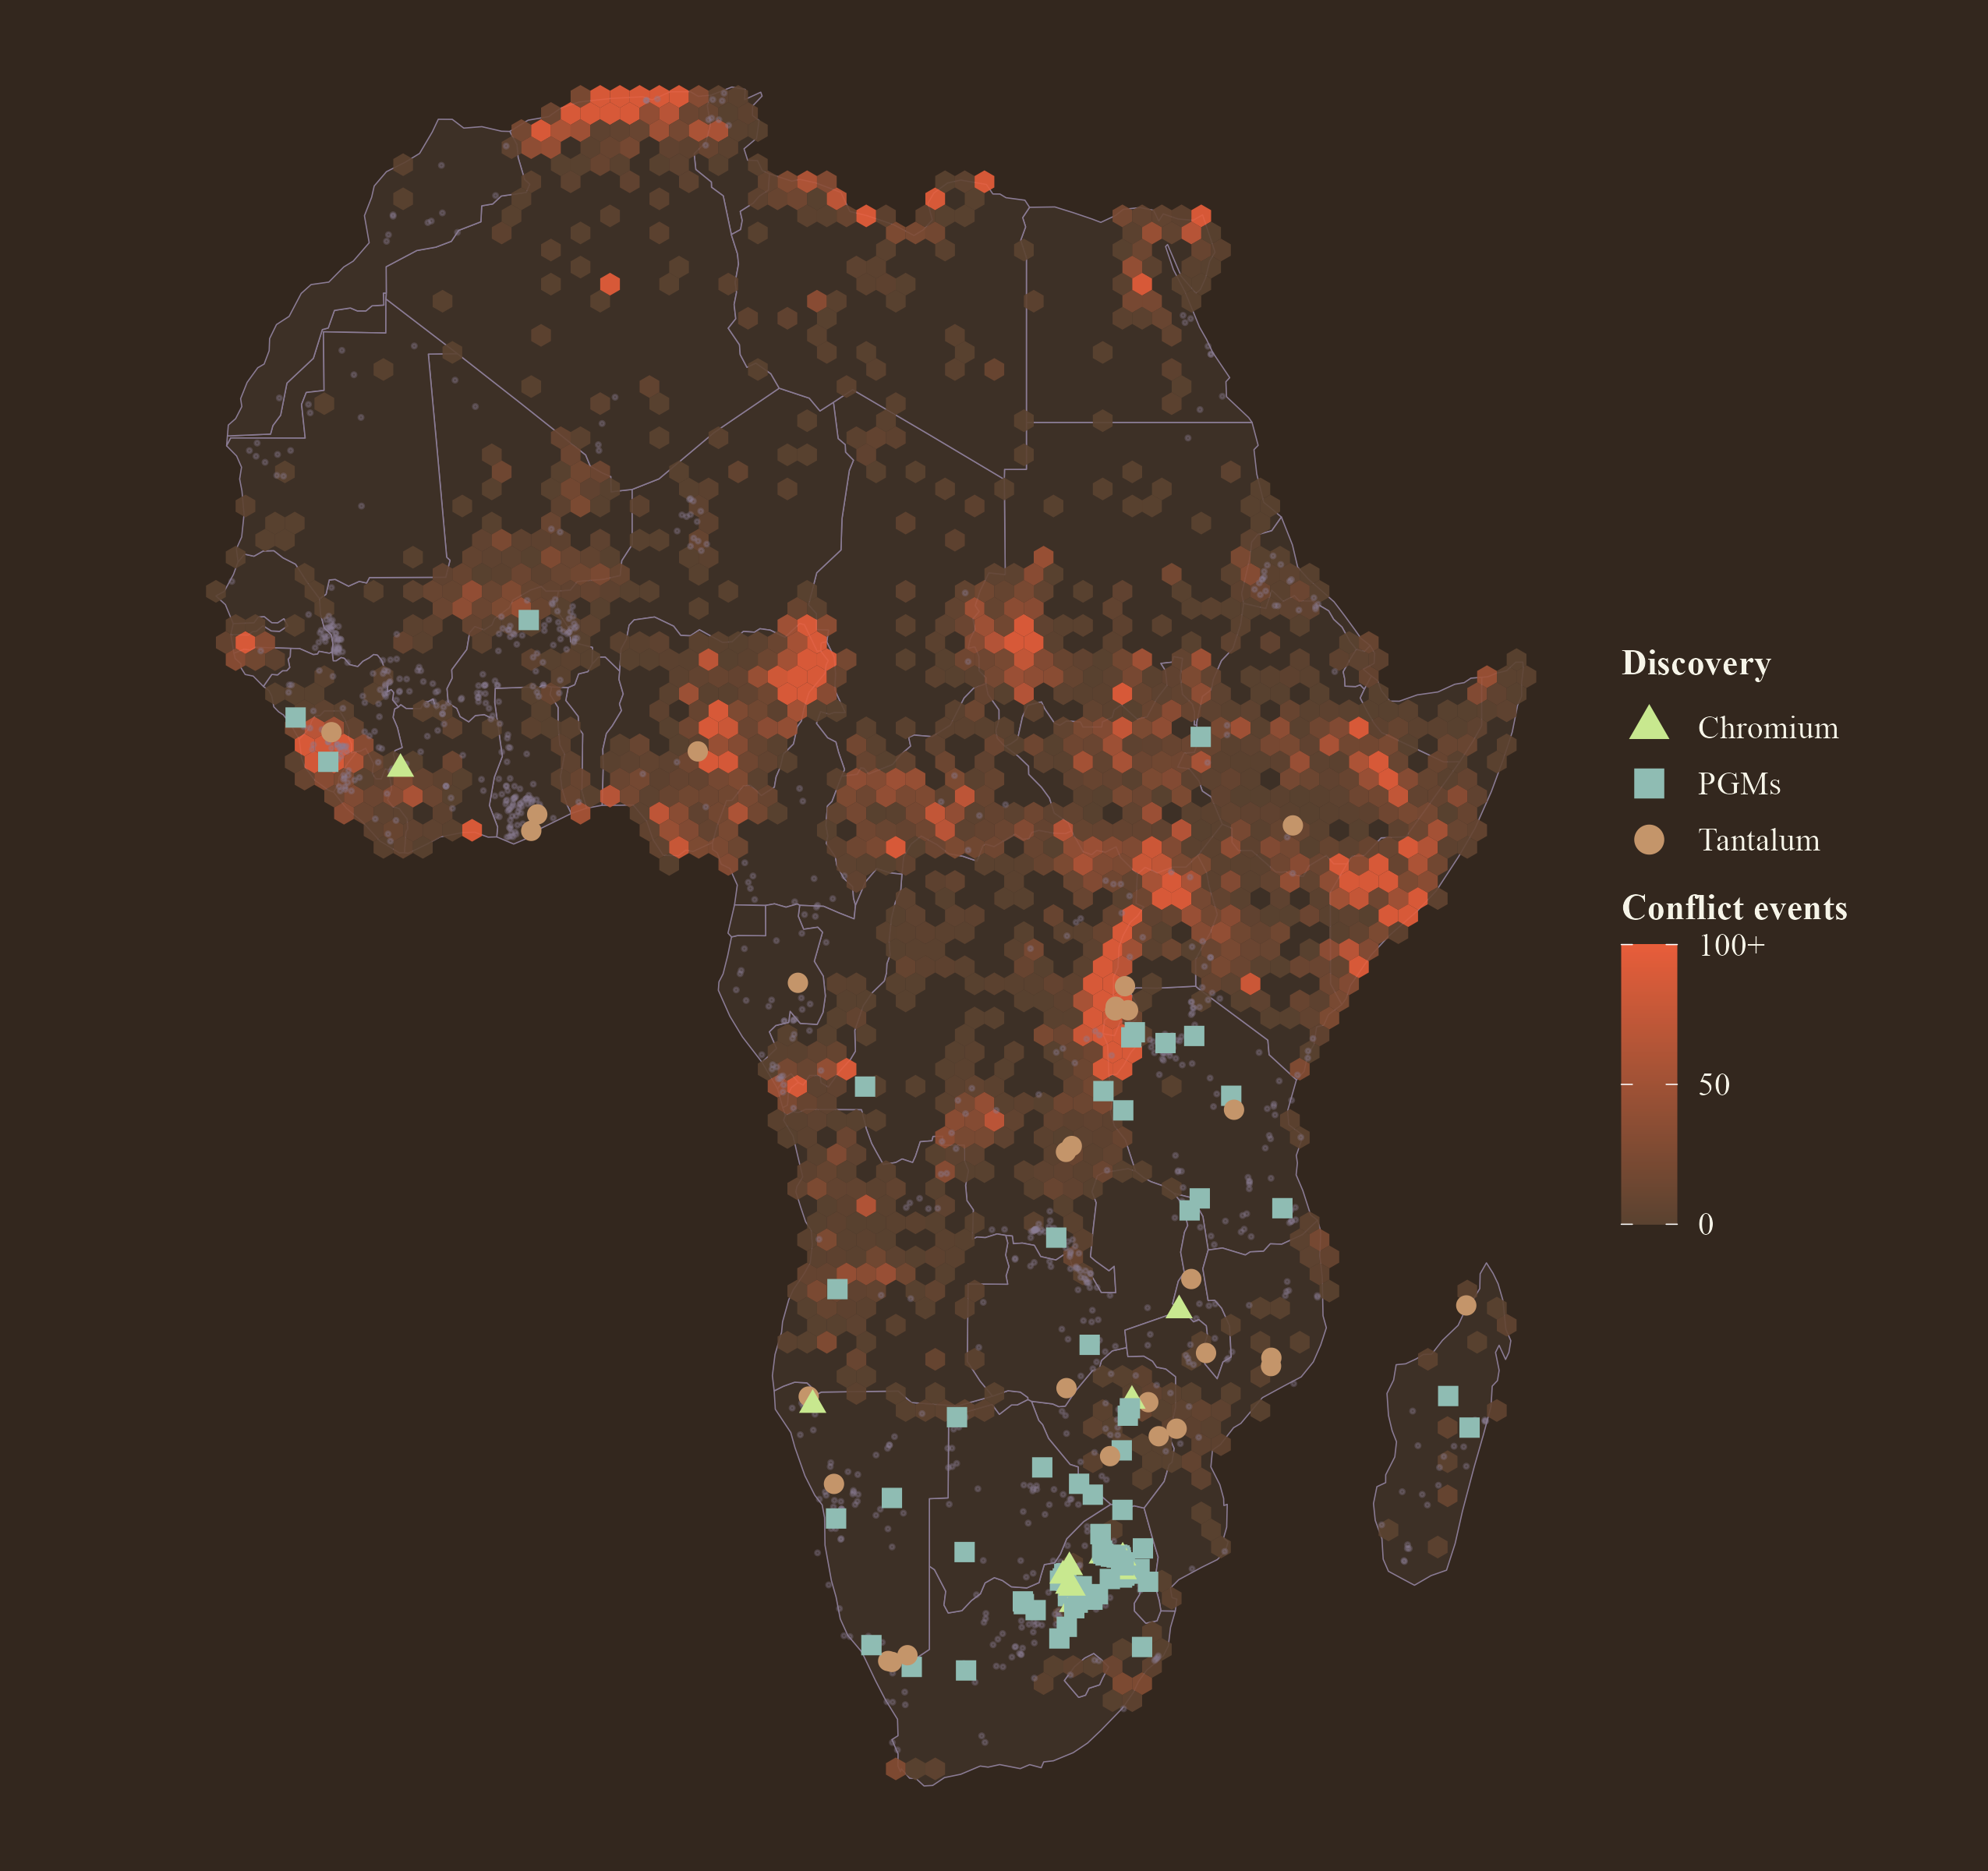
\includegraphics[width=\textwidth]{plots/deck/map_dark.png}
    \end{column}
  \end{columns}
\end{frame}

% ═══════════════════════════════ MOTIVATION ═════════════════════════════
\begin{frame}{Why It Matters Now}
  \begin{columns}[T]
    \begin{column}{0.55\textwidth}
      \begin{itemize}
        \item The energy transition is driving demand for minerals concentrated in
              conflict-prone regions
        \item Africa holds much of the supply
        \item Governance is \textbf{wildly uneven}: some minerals sit under
              international due diligence regimes, some under strong national law,
              some under nothing at all
      \end{itemize}
    \end{column}
    \begin{column}{0.45\textwidth}
      \begin{block}{The policy payoff}
        Dodd--Frank 1502, ITSCI and the OECD Guidance assume that cutting armed
        groups off from mineral revenue makes these places safer.
      \end{block}
      \vspace{0.5em}
      {\color{lime}We test that assumption.}
    \end{column}
  \end{columns}
\end{frame}

% ═══════════════════════════════ THEORY ═════════════════════════════════
\begin{frame}{Three Governance Regimes}
  \begin{columns}[T]
    \begin{column}{0.33\textwidth}
      \begin{block}{International}
        \textcolor{sand}{\textbf{Tantalum}}\\[0.3em]
        {\small Dodd--Frank 1502, ITSCI, OECD. Transparency and traceability
        cut off armed group financing.}
      \end{block}
    \end{column}
    \begin{column}{0.33\textwidth}
      \begin{block}{National}
        \textcolor{sage}{\textbf{PGMs}}\\[0.3em]
        {\small South Africa's MPRDA. State custodianship and licensing;
        industrial extraction excludes informal actors.}
      \end{block}
    \end{column}
    \begin{column}{0.33\textwidth}
      \begin{block}{Governance gap}
        \textcolor{lime}{\textbf{Chromium}}\\[0.3em]
        {\small No equivalent regime. High strategic value, no transparency
        requirement, no certification.}
      \end{block}
    \end{column}
  \end{columns}
  \vspace{1em}
  \begin{center}
    {\color{sage}The effect of discovery should depend on which regime applies.}
  \end{center}
\end{frame}

\begin{frame}{Hypotheses}
  \vspace{0.4em}
  {\small Each regime gets a prediction about \textbf{how often} violence happens
  and one about \textbf{how deadly} it is.}
  \vspace{0.9em}
  \begin{itemize}\setlength\itemsep{0.35em}
    \item[\textcolor{sand}{\textbf{H1a}}] International governance
          \textbf{reduces conflict events}
    \item[\textcolor{sand}{\textbf{H1b}}] International governance
          \textbf{reduces battle deaths}
    \item[\textcolor{sage}{\textbf{H2a}}] National governance
          \textbf{reduces conflict events}
    \item[\textcolor{sage}{\textbf{H2b}}] National governance
          \textbf{reduces battle deaths}
    \item[\textcolor{lime}{\textbf{H3a}}] Governance gap
          \textbf{increases conflict events}
    \item[\textcolor{lime}{\textbf{H3b}}] Governance gap
          \textbf{increases battle deaths}
  \end{itemize}
  \vspace{0.7em}
  {\small\color{muted}Each follows from a different mechanism. Certification
  defunds armed groups. State monopoly formalises extraction. Absent oversight,
  high value and no scrutiny should invite contestation \textemdash{} the
  standard resource-curse expectation.}
\end{frame}

% ═══════════════════════════════ DATA ═══════════════════════════════════
\begin{frame}{Data}
  \begin{columns}[T]
    \begin{column}{0.5\textwidth}
      \textbf{Discoveries} \\[0.3em]
      {\small S\&P Global Market Intelligence. 1{,}093 African exploration sites
      across 42 countries, 1995--2018.}
      \vspace{0.7em}

      {\small Treatment is the \textbf{first year a cell records exploration
      activity} for the mineral.}
      \vspace{1.0em}

      \textbf{Sample} \\[0.3em]
      {\small Tantalum and PGM samples are cut to when their governance regimes
      were first established. Chromium has none, so it uses the full panel.}
    \end{column}
    \begin{column}{0.5\textwidth}
      \textbf{Conflict} \\[0.3em]
      {\small UCDP-GED v25.1. Events and battle deaths, plus the Actor Dataset
      for who initiates violence and who is targeted by it.}
      \vspace{1.0em}

      \textbf{Unit of analysis} \\[0.3em]
      {\small Hexagonal grid cells at seven resolutions, 25--300\,km.
      Main analysis at 100\,km: 3{,}658 cells, 87{,}792 cell-years.}
    \end{column}
  \end{columns}
\end{frame}

% ═══════════════════════════════ METHODS ════════════════════════════════
\begin{frame}{Design}
  \begin{itemize}
    \item Staggered difference-in-differences, \textbf{Callaway--Sant'Anna}
    \item Cells treated at different times; never-treated cells as controls
  \end{itemize}
  \vspace{0.8em}
  \begin{block}{Two features that shape how we read it}
    \begin{itemize}
      \item Effects \textbf{emerge slowly}. Little happens before year five.
      \item The later window is identified from the \textbf{earliest cohorts},
            so it rests on fewer cells.
    \end{itemize}
  \end{block}
  \vspace{0.4em}
\end{frame}

% ═══════════════════════════════ RESULTS ════════════════════════════════
\begin{frame}[standout]
  Main results
\end{frame}

\begin{frame}{Effects by Governance Regime}
  \begin{center}
    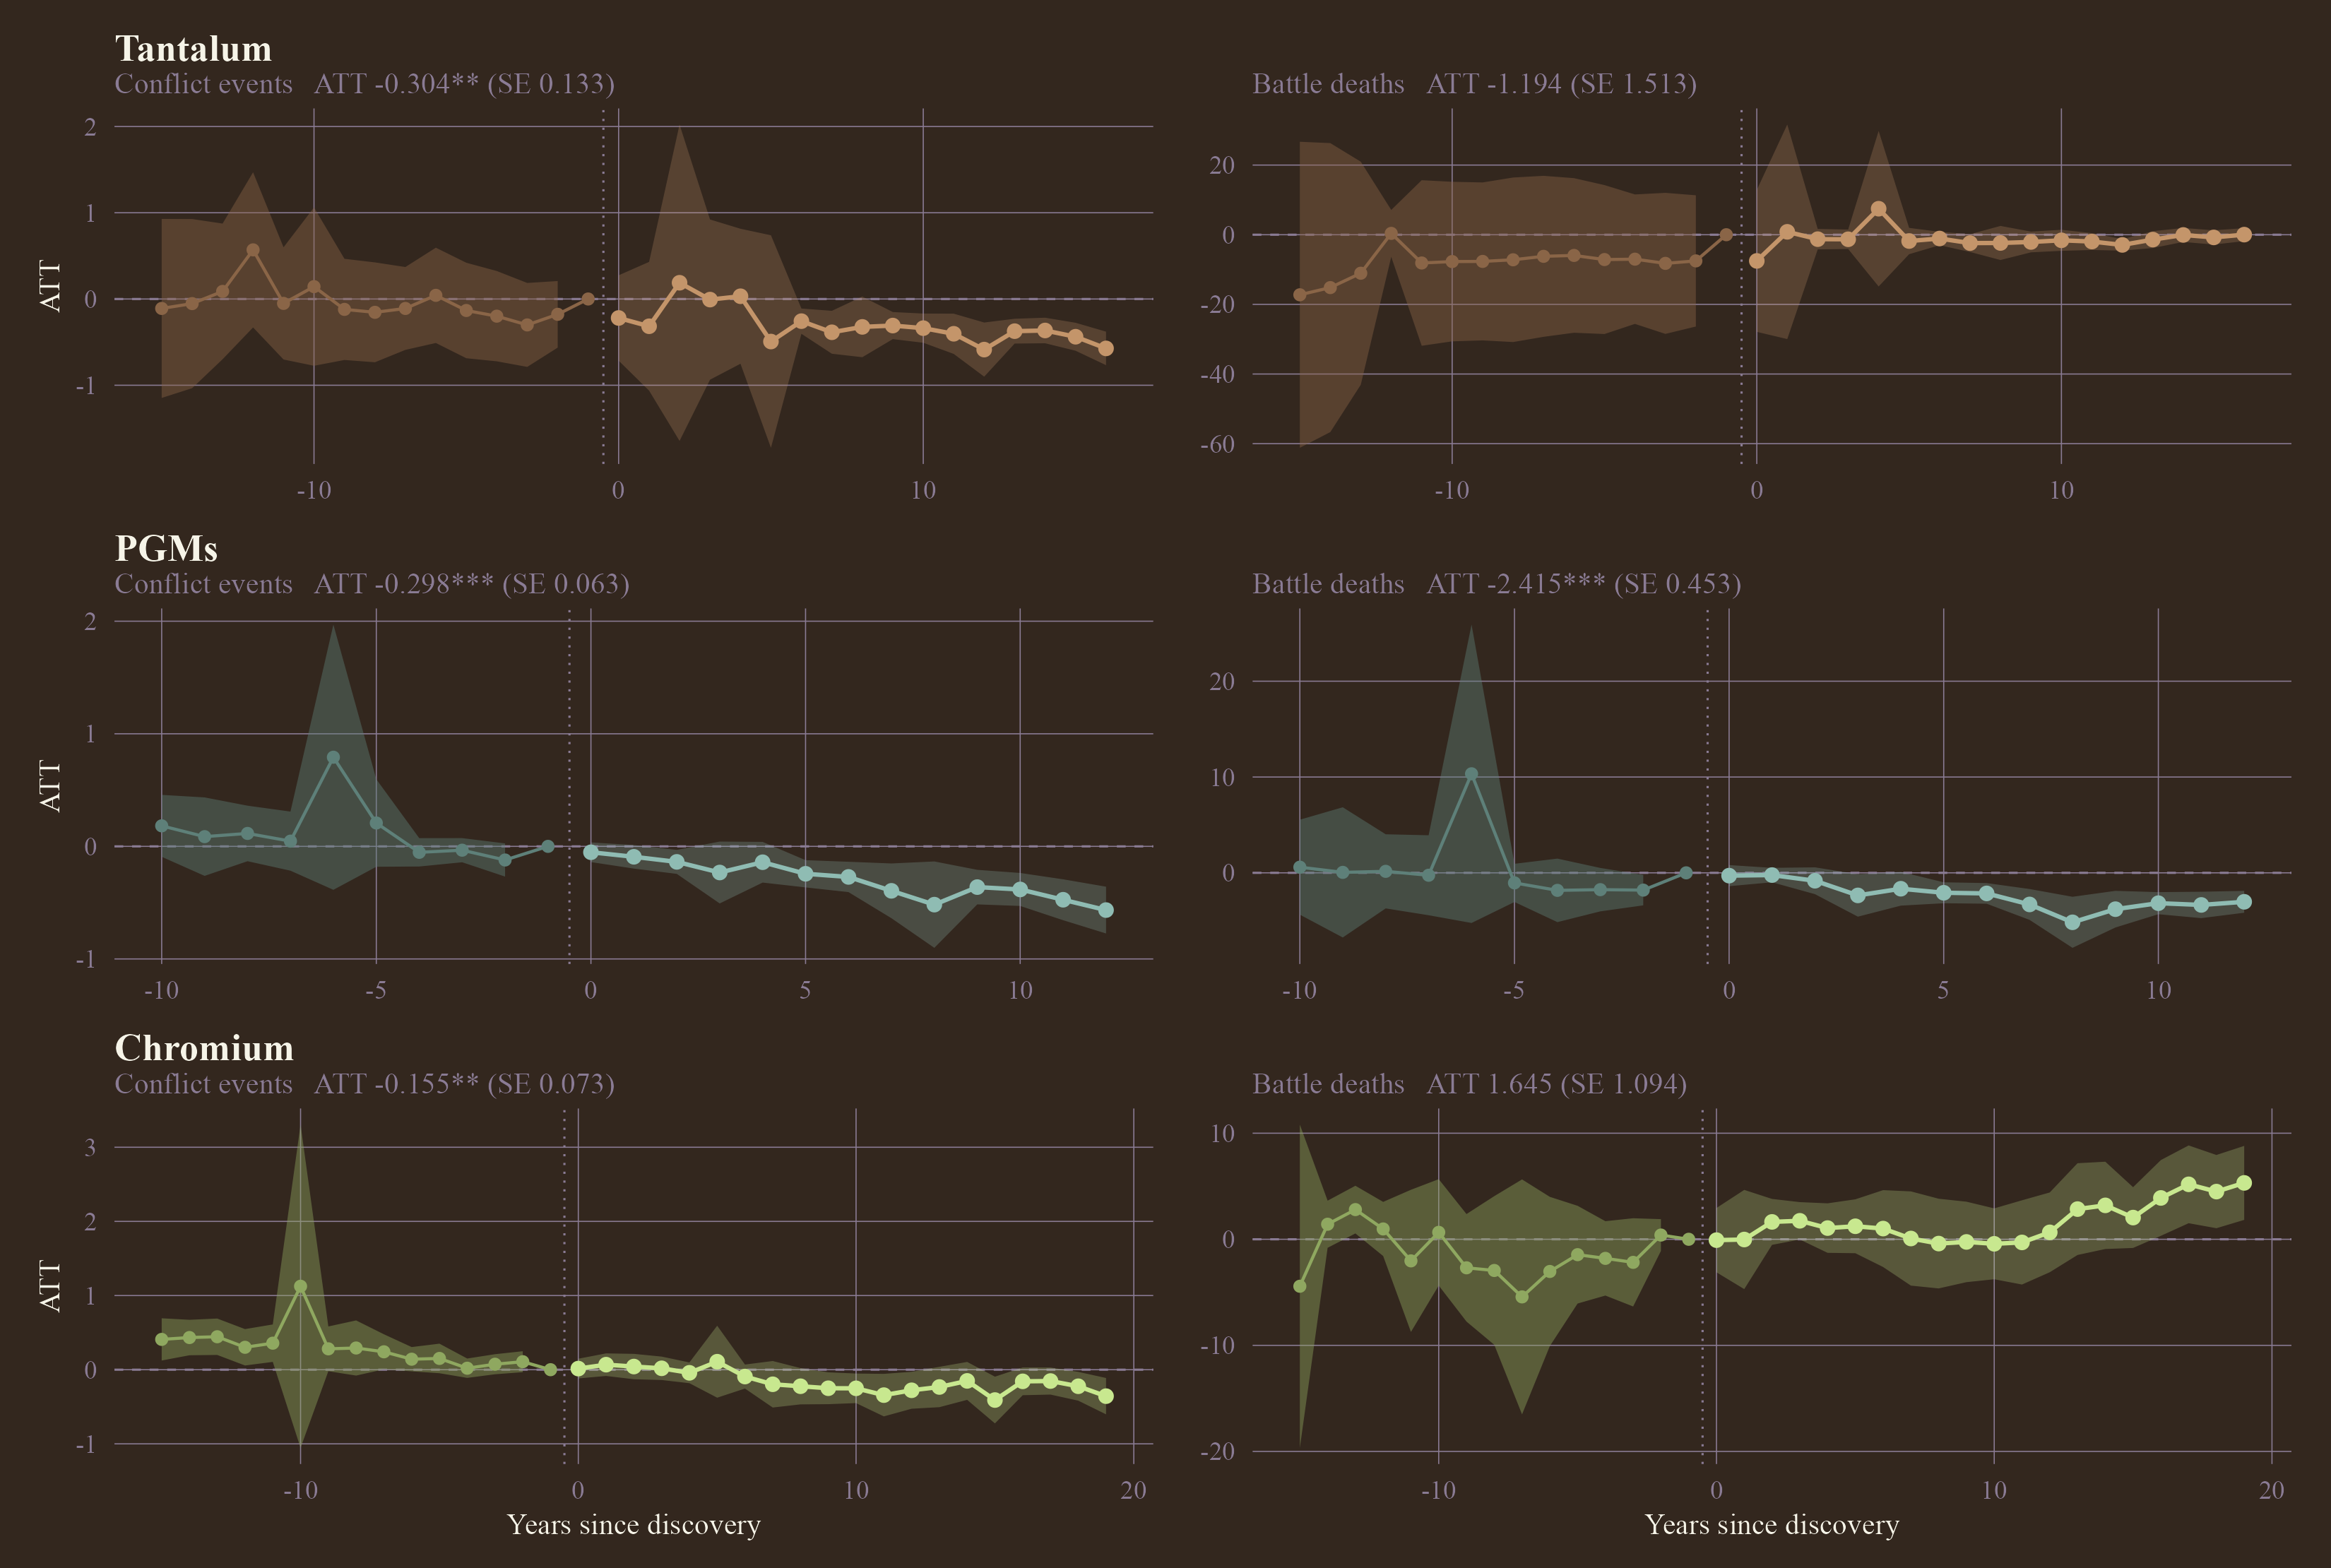
\includegraphics[width=0.80\textwidth]{plots/deck/regime_final_dark.png}
  \end{center}
\end{frame}

\begin{frame}{What the Results Say}
  \vspace{0.3em}
  \begin{center}
  {\small
  \begin{tabular}{llcc}
    \toprule
    \textbf{Mineral} & \textbf{Regime}
      & \textbf{Conflict events} & \textbf{Battle deaths} \\
    \midrule
    \textcolor{sand}{Tantalum} & International
      & $\downarrow$ $-0.30^{**}$  & $-1.19$ \\[0.25em]
    \textcolor{sage}{PGMs} & National
      & $\downarrow$ $-0.30^{***}$ & $\downarrow$ $-2.42^{***}$ \\[0.25em]
    \textcolor{lime}{Chromium} & Gap
      & $\downarrow$ $-0.16^{**}$  & $\uparrow$ $+1.65$ \\
    \bottomrule
  \end{tabular}}
  \end{center}
  \vspace{0.2em}
  {\scriptsize\color{muted}Dynamic Callaway--Sant'Anna aggregates, 100\,km.
  $^{*}p<0.10$, $^{**}p<0.05$, $^{***}p<0.01$. Chromium battle deaths reach
  $+2.69^{**}$ from the tenth post-treatment year.}
  \vspace{0.8em}

  \begin{columns}[T]
    \begin{column}{0.5\textwidth}
      {\small\color{sage}\textbf{Events fall under all three regimes.}\\
      H1a and H2a supported. \textbf{H3a is contradicted}: we expected the
      governance gap to invite contestation, and found the opposite.}
    \end{column}
    \begin{column}{0.5\textwidth}
      {\small\color{lime}\textbf{Lethality is where they differ.}\\
      H2b and H3b supported. \textbf{H1b is not} \textemdash{} international
      governance does not reduce deaths.}
    \end{column}
  \end{columns}
\end{frame}

\begin{frame}[standout]
  Mechanisms
\end{frame}

\begin{frame}{Armed Groups Leave}
  \begin{center}
    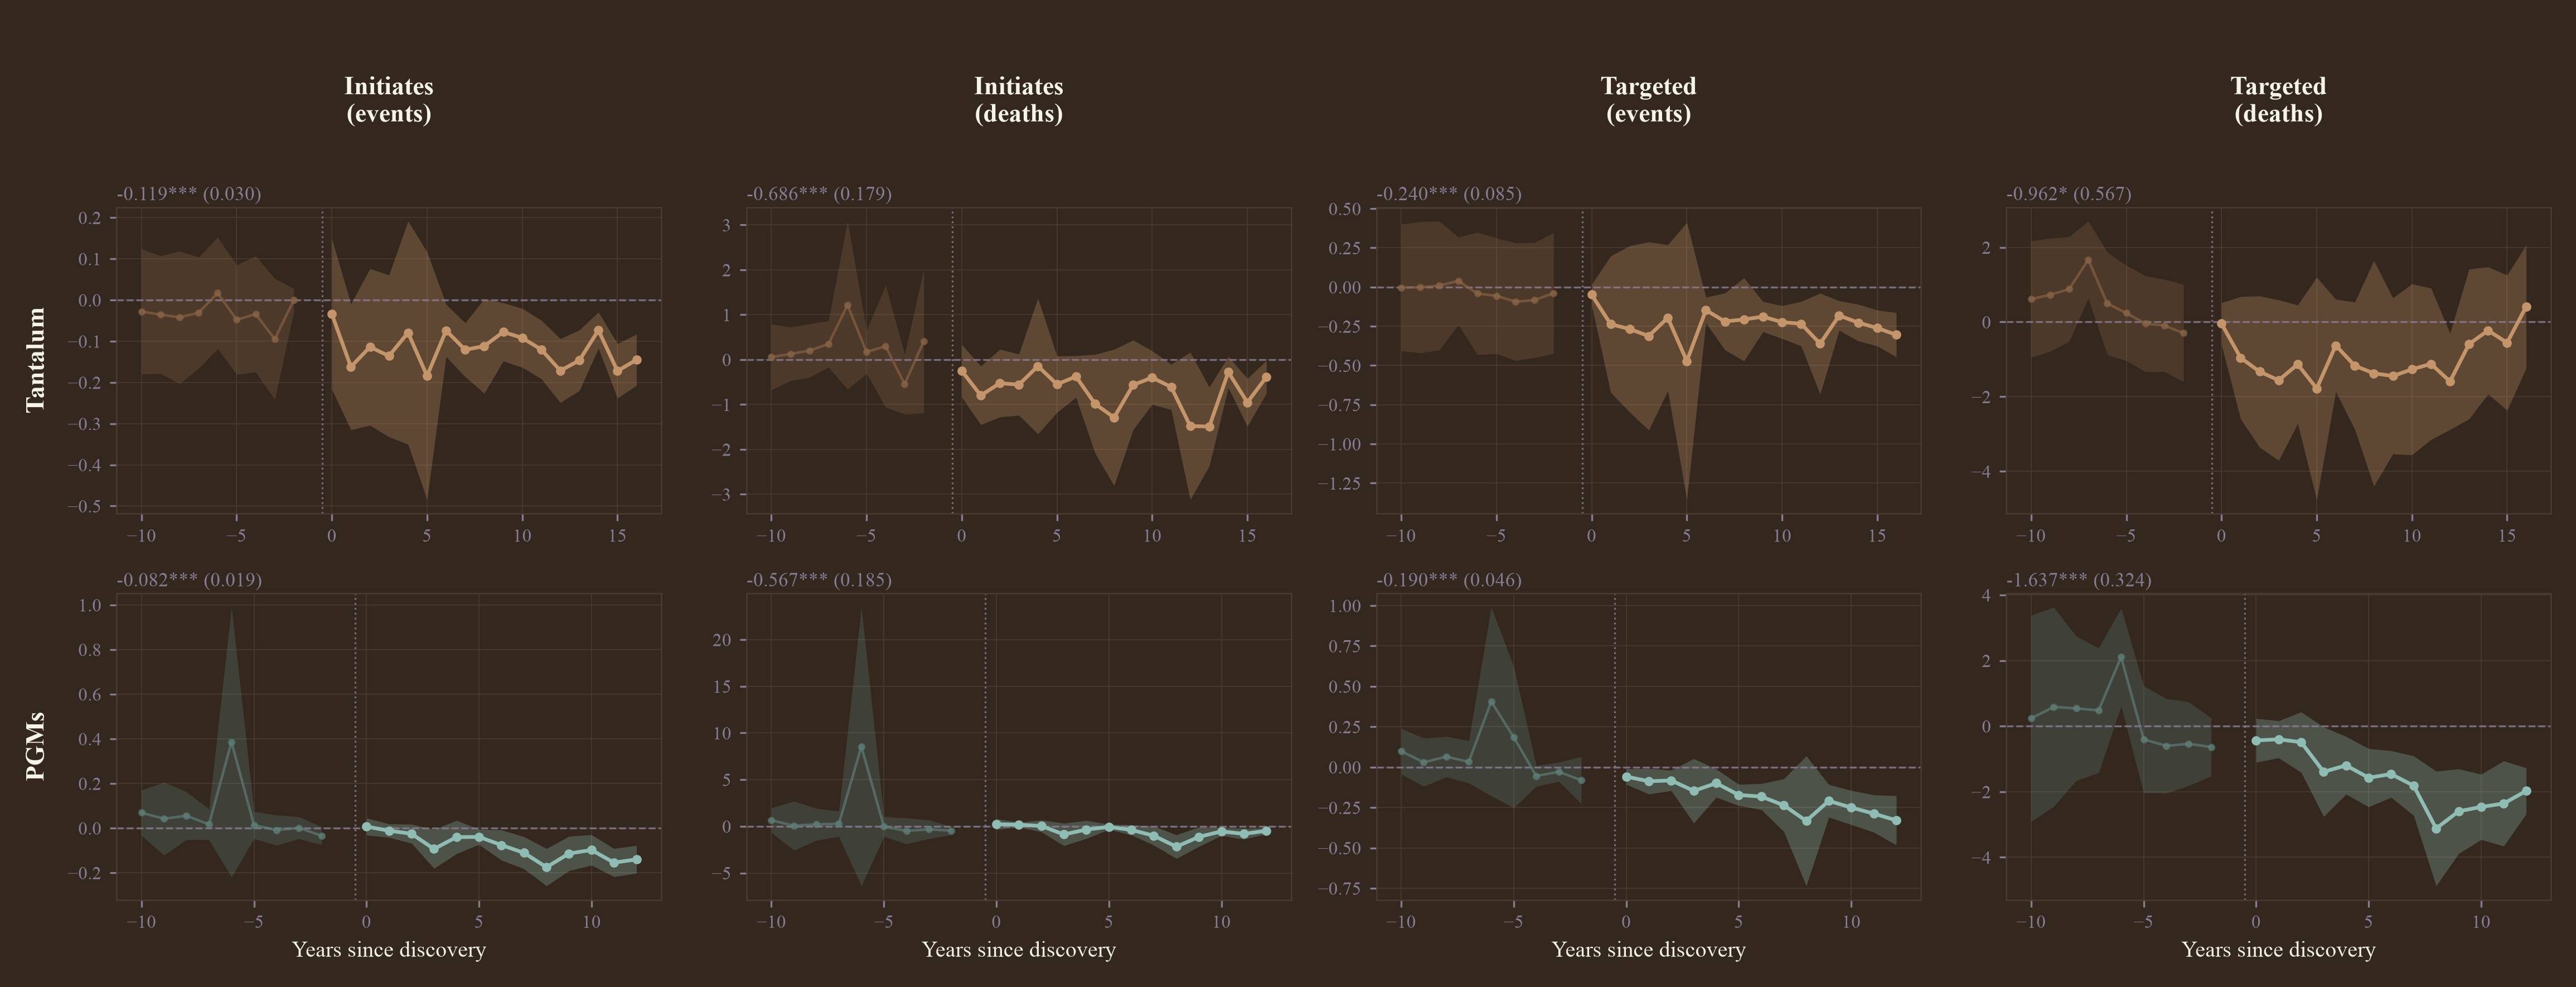
\includegraphics[width=\textwidth]{plots/deck/rebels_dark.png}
  \end{center}
  \vspace{-0.4em}
  {\scriptsize\color{muted}Formal armed groups decline under both governed
  regimes, as initiators and as targets.}
\end{frame}

\begin{frame}{Who Holds the Deposit Afterwards? The State}
  \vspace{0.2em}
  \begin{columns}[T]
    \begin{column}{0.33\textwidth}
      \vspace{0.6em}
      {\small
      \begin{itemize}\setlength\itemsep{0.55em}
        \item State-initiated \textbf{events fall} under all three regimes.
        \item \textcolor{sand}{Deaths stay flat} where governance is
              international.
        \item \textcolor{sage}{Deaths fall} where it is national.
        \item \textcolor{lime}{Deaths climb} from about the tenth year where
              there is no regime.
      \end{itemize}}
    \end{column}
    \begin{column}{0.67\textwidth}
      \centering
      \raisebox{-\height}{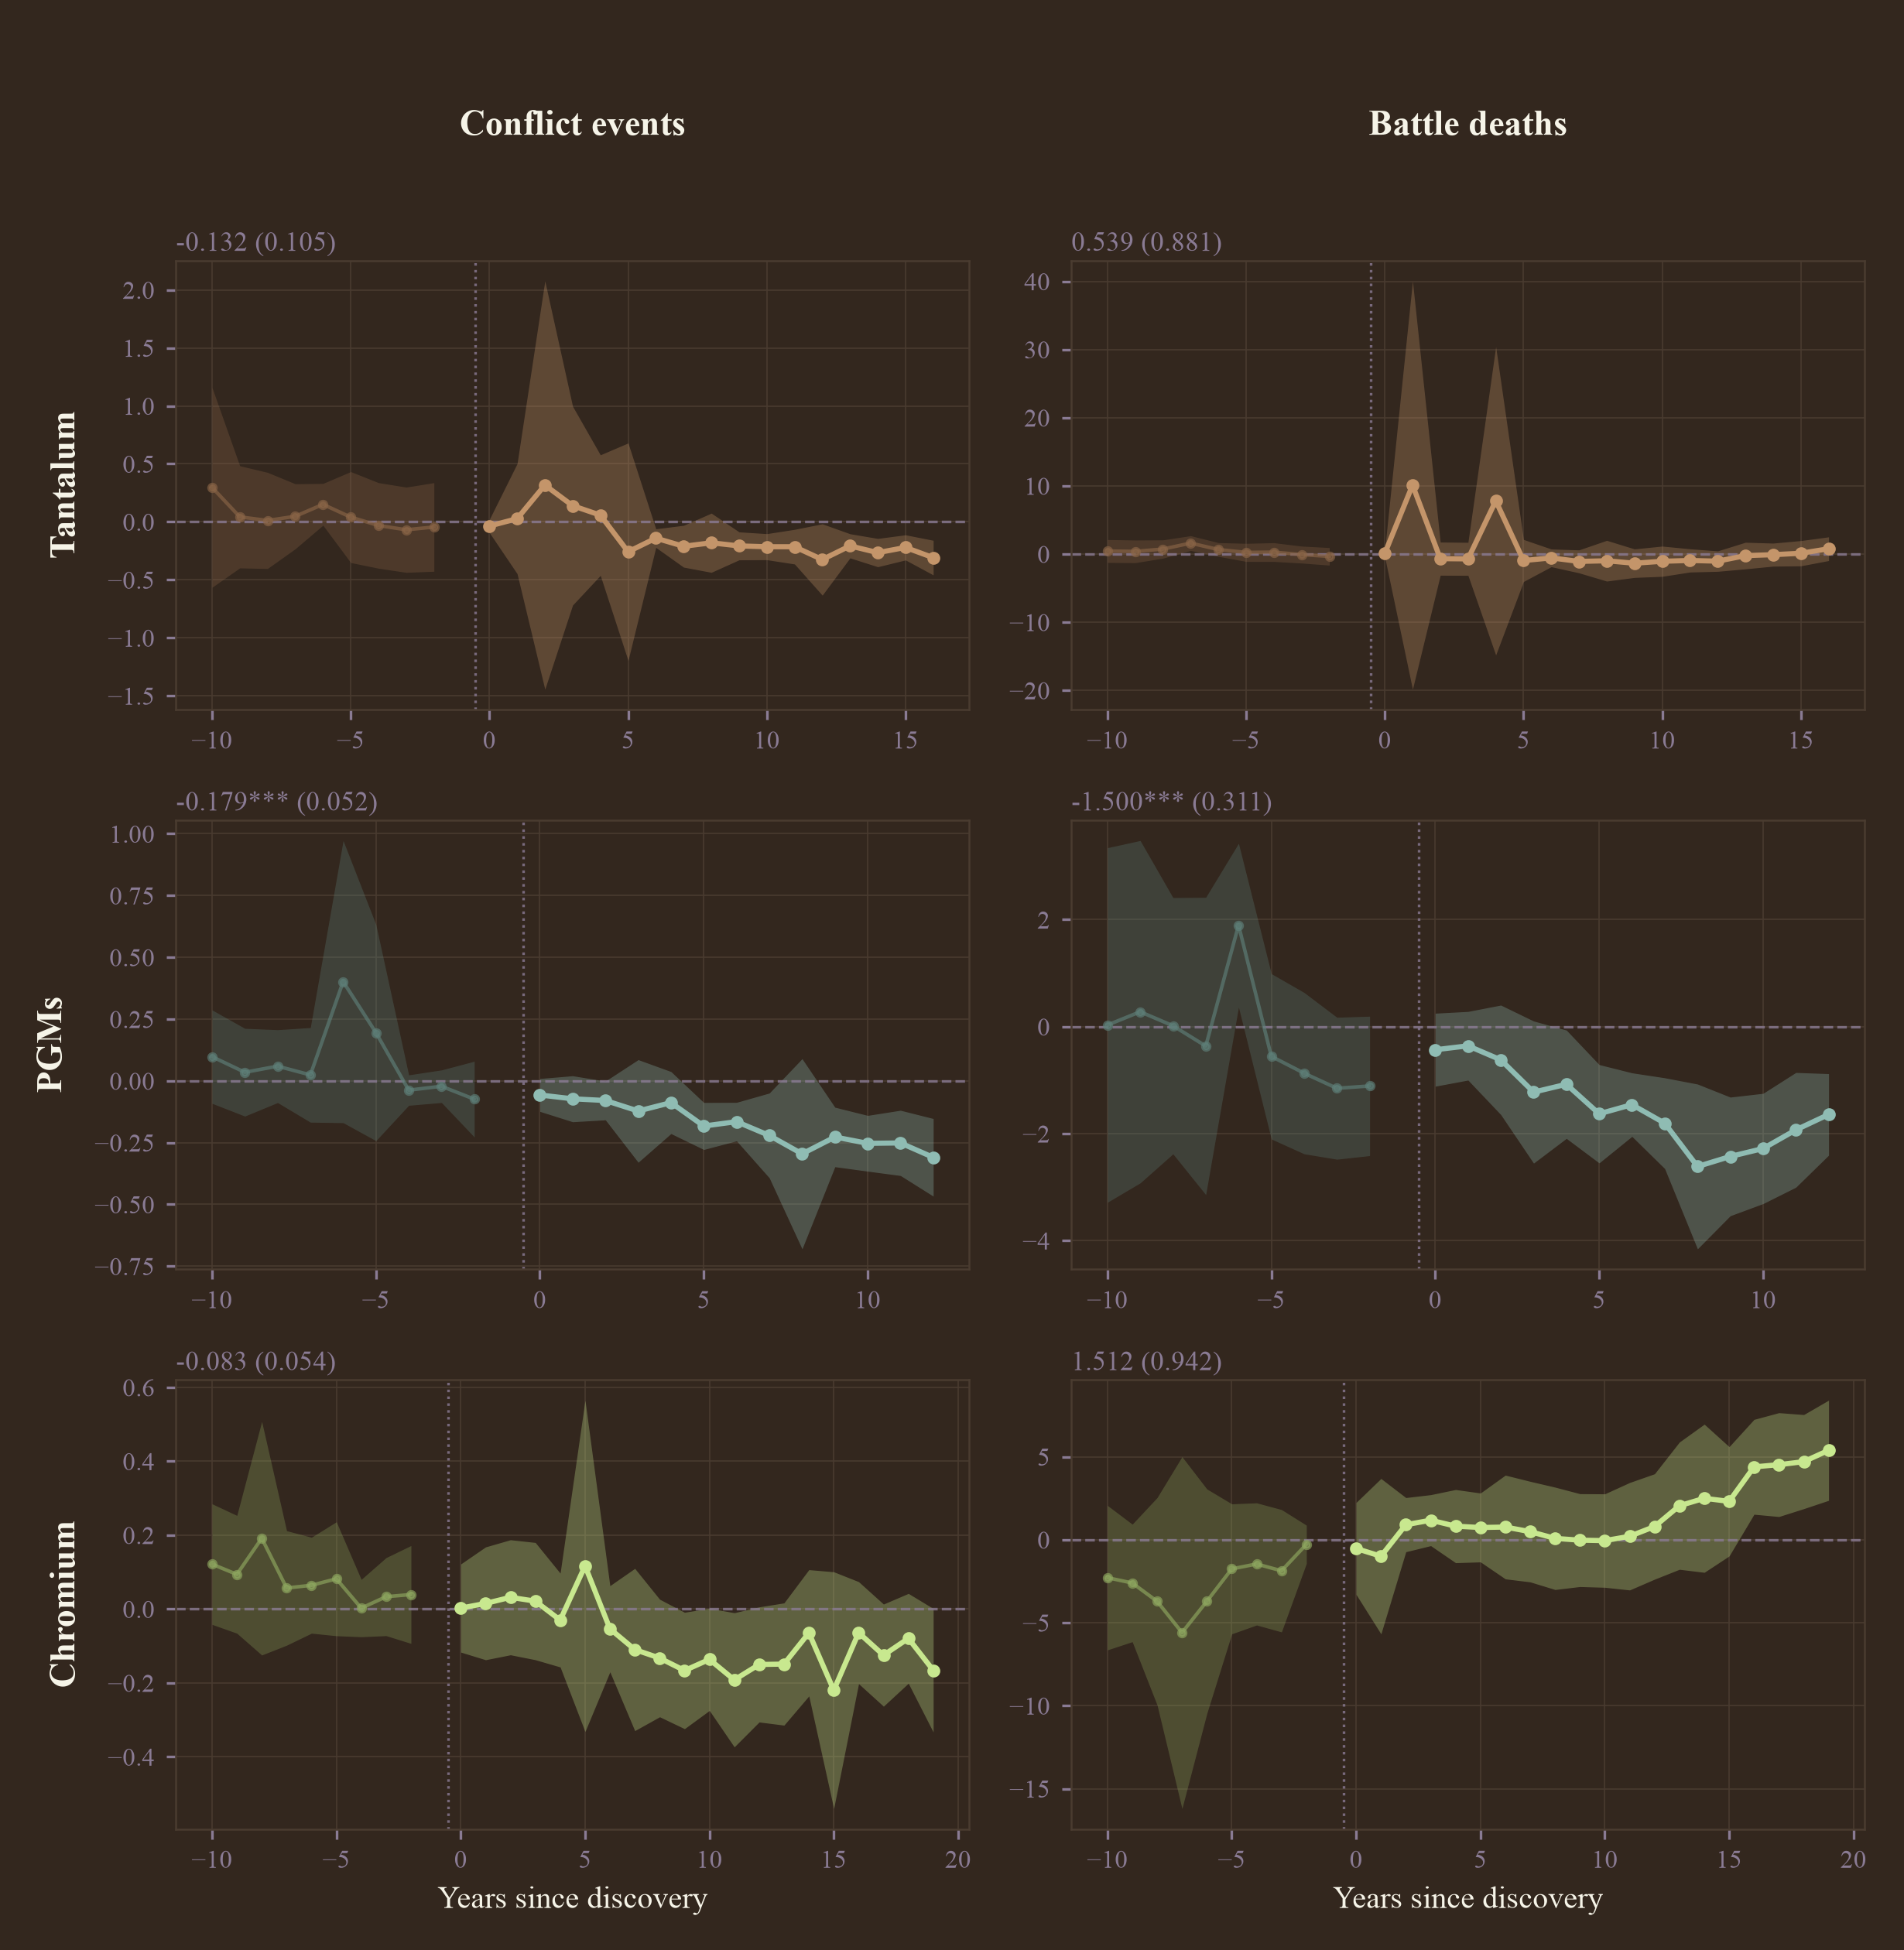
\includegraphics[height=0.90\textheight]{plots/deck/state_dark.png}}
    \end{column}
  \end{columns}
\end{frame}

\begin{frame}{Civilians}
  \vspace{0.2em}
  \begin{columns}[T]
    \begin{column}{0.33\textwidth}
      \vspace{0.6em}
      {\small
      \begin{itemize}\setlength\itemsep{0.55em}
        \item Civilian outcomes \textbf{track the state panel} almost exactly.
        \item That is what we would expect if the state is the actor that
              remains once armed groups withdraw.
        \item The same ordering holds: \textcolor{sand}{flat},
              \textcolor{sage}{down}, \textcolor{lime}{up}.
      \end{itemize}}
    \end{column}
    \begin{column}{0.67\textwidth}
      \centering
      \raisebox{-\height}{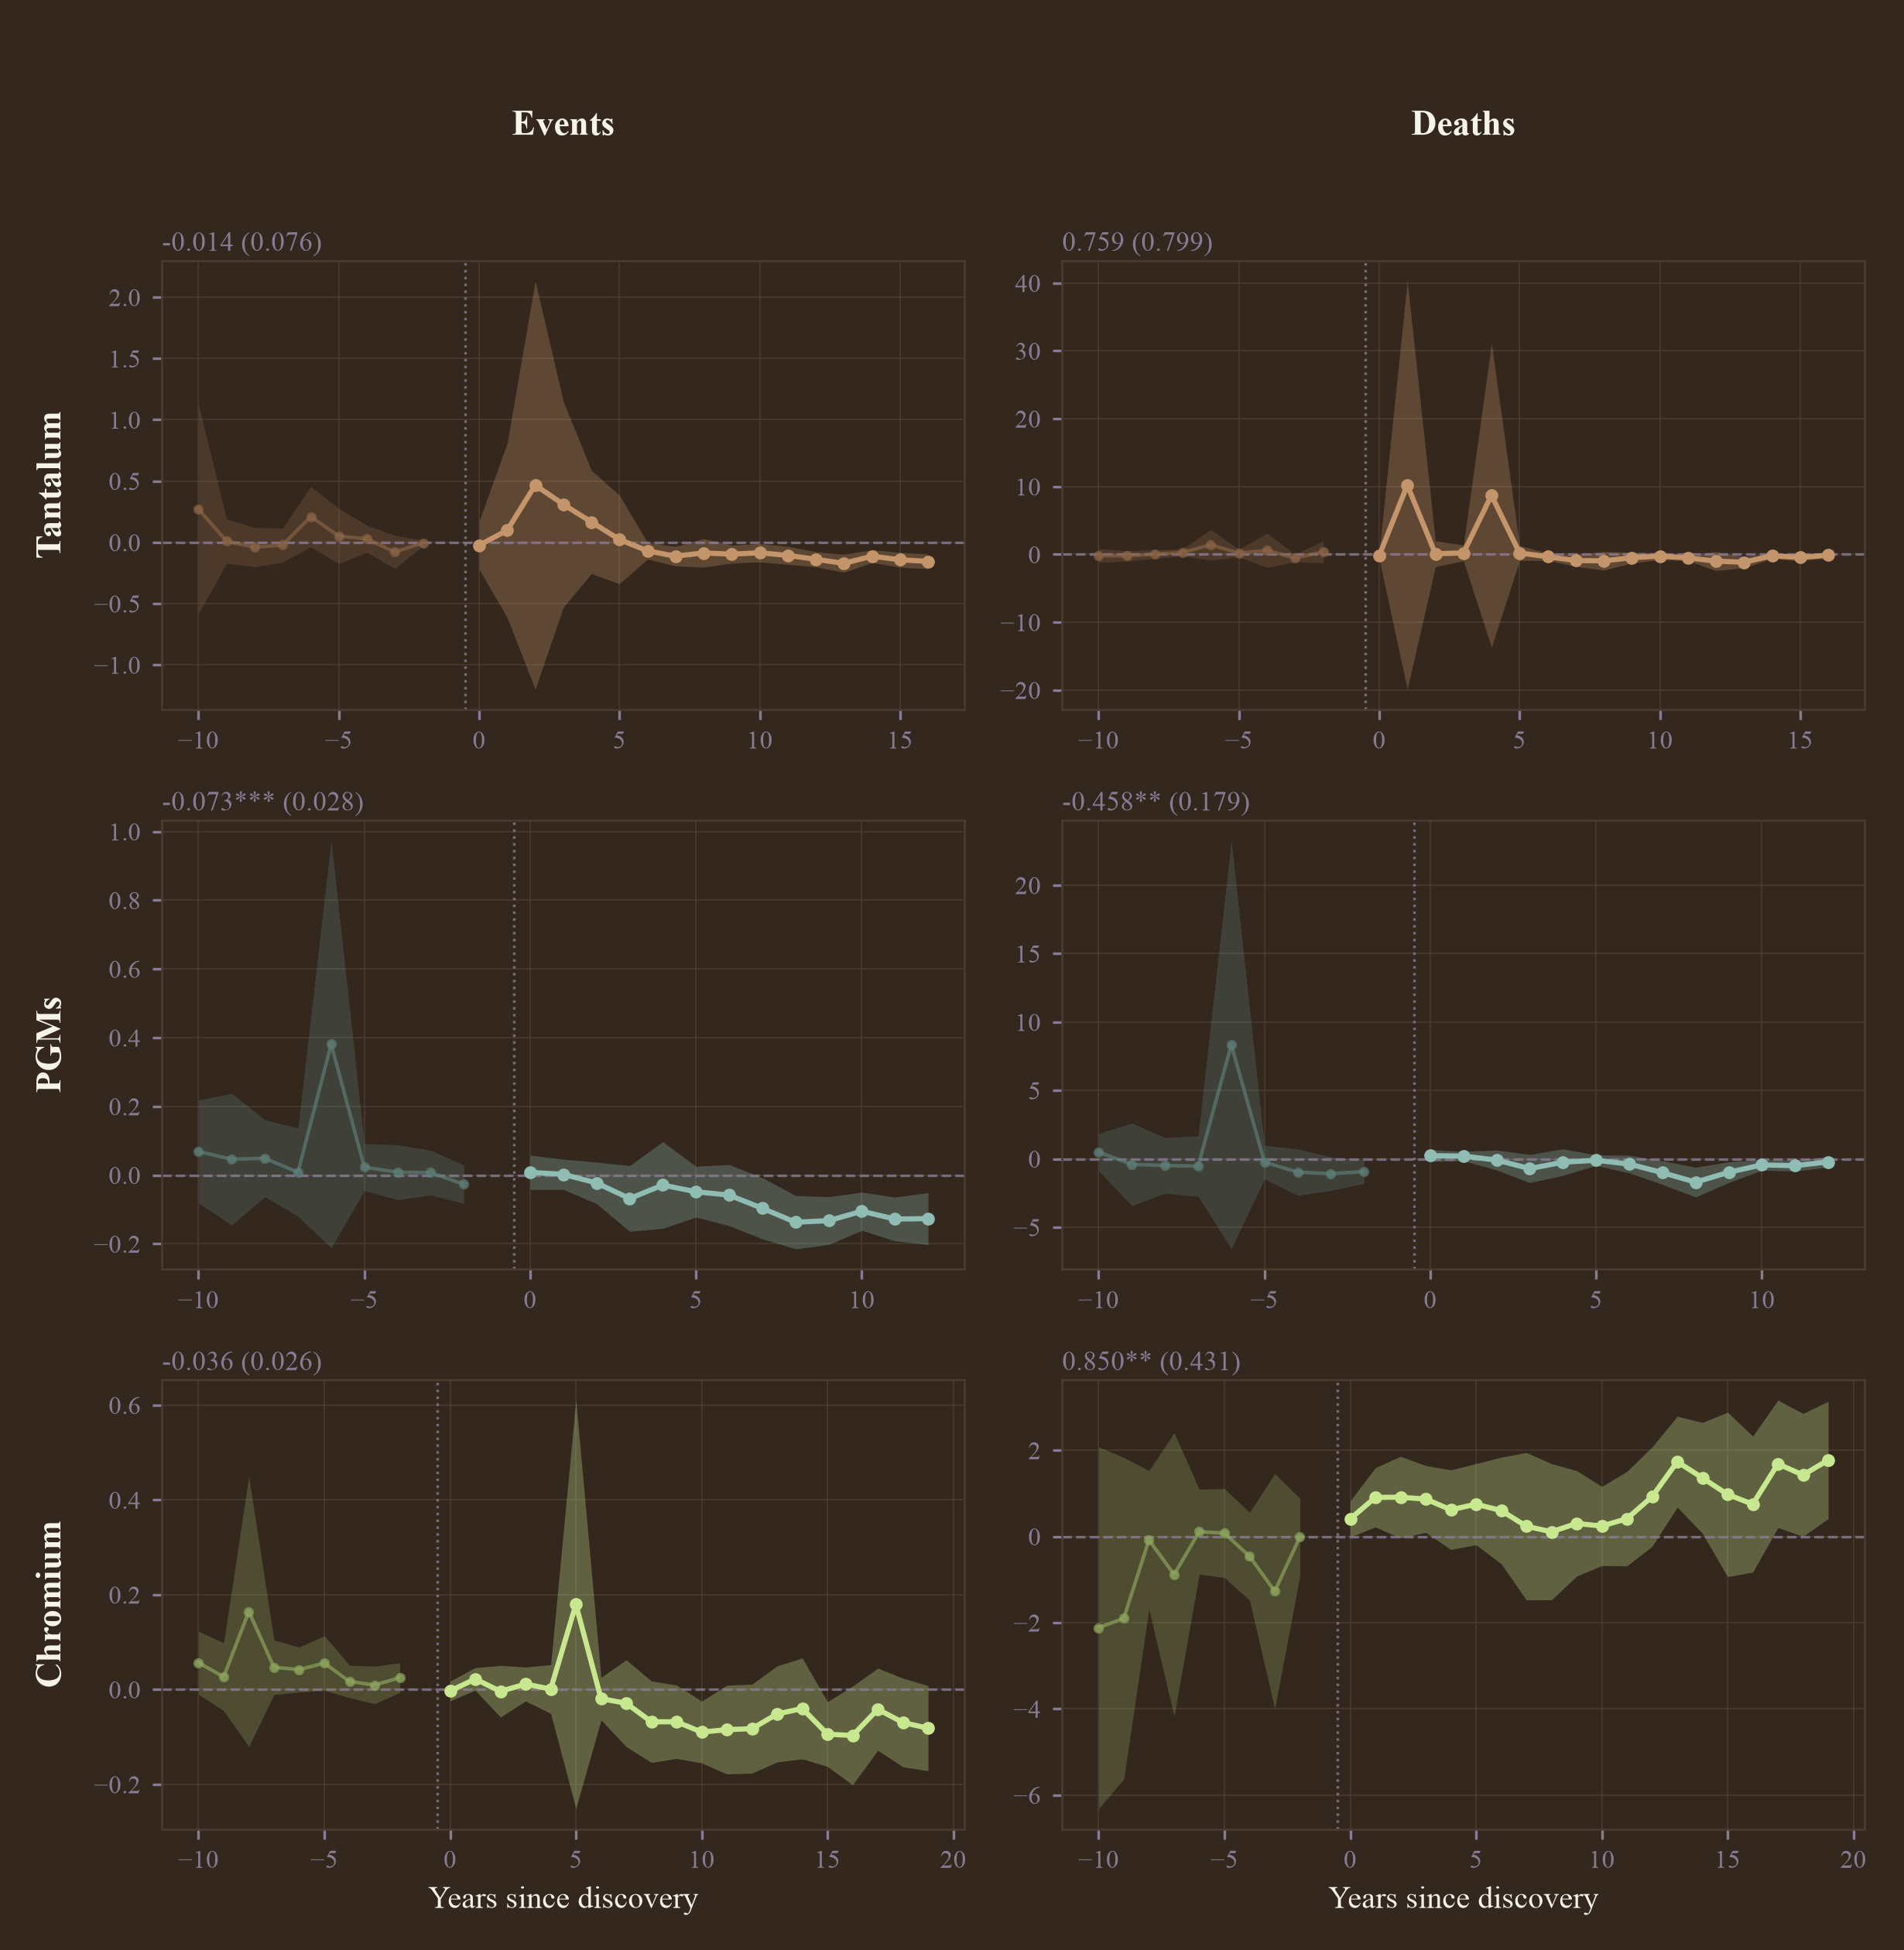
\includegraphics[height=0.90\textheight]{plots/deck/civilians_dark.png}}
    \end{column}
  \end{columns}
\end{frame}

\begin{frame}{Conclusions}
  \vspace{0.4em}
  \begin{itemize}\setlength\itemsep{0.35em}
    \item \textcolor{lime}{\textbf{We expected ungoverned deposits to invite
          contestation. They do not.}} Conflict events fall there too. Chromium
          extraction is industrial, so it offers armed groups no foothold, and
          there is no certification regime worth capturing.
    \item \textbf{Discovery reduces how often violence happens, under every
          regime.} That does not distinguish them.
    \item \textbf{Lethality does.} Deaths fall under national governance, do not
          move under international governance, and rise where there is no regime.
    \item \textbf{The difference is not how much governance, but whether state
          control is constrained.} Licensed extraction reduces killing. The same
          state securing an unregulated deposit does not.
    \item \textbf{Lootability cannot explain this.} PGMs and chromium are both
          industrial, both largely South African, and they diverge.
  \end{itemize}
  \vspace{0.5em}
  {\small\color{muted}\textbf{Next.} Separating governance from extraction mode,
  and following these minerals from discovery into production.}
\end{frame}

\begin{frame}[standout]
  \begin{center}
    {\Large Thank you}
    \vspace{1.6em}

    {\normalsize
     Elisa D'Amico \quad {\small\ttfamily elisa.damico@ucd.ie}\\[0.5em]
     P\"aivi Lujala \quad {\small\ttfamily Paivi.Lujala@oulu.fi}}
    \vspace{1.2em}

    {\small University College Dublin \quad\textbullet\quad University of Oulu}
  \end{center}
\end{frame}

\end{document}
